\documentclass[12pt]{article}
\usepackage[margin=30mm]{geometry}
\usepackage{todonotes}
\usepackage{pdfpages}
\usepackage{graphicx}
\usepackage{url}
\usepackage[parfill]{parskip}
\usepackage{verbatim}
\usepackage{listings}
\usepackage{color}

\usepackage [english]{babel}
\usepackage [autostyle, english = american]{csquotes}
\MakeOuterQuote{"}

\definecolor{dkgreen}{rgb}{0,0.6,0}
\definecolor{gray}{rgb}{0.5,0.5,0.5}
\definecolor{mauve}{rgb}{0.58,0,0.82}

\lstset{frame=tb,
  language=Python,
  aboveskip=3mm,
  belowskip=3mm,
  showstringspaces=false,
  columns=flexible,
  basicstyle={\small\ttfamily},
  numbers=none,
  numberstyle=\tiny\color{gray},
  keywordstyle=\color{blue},
  commentstyle=\color{dkgreen},
  stringstyle=\color{mauve},
  breaklines=true,
  breakatwhitespace=true,
  tabsize=3
}

\begin{document}
\title{Advanced Topics in Software Engineering - Handin 3}
\author{Jack Neilson}
\maketitle
\newpage


\section{Introduction}
Deciding what features to implement on the next release of a piece of software is a difficult problem, particularly if the software has a large user base. The company making the software must decide what customers it prioritises, the benefit each requirement will have to each customer, the cost (in both time and money) of each requirement, and the budget they have. When considering these objectives, it is impossible to optimise each one - a tradeoff must be considered where the benefit of implementing a requirement is balanced against the cost. With a non-trivial set of requirements the entire search space cannot be enumerated, as the problem of multiple objective search is NP-complete.

A potential solution to this problem is to use a genetic algorithm which can optimise for 2 or more objectives. This report will demonstrate the NSGA-II algorithm for the problem of next-release requirements, with a comparison of a single-objective genetic algorithm and a random search.


\section{NSGA-II Description}
The NSGA-II algorithm works by taking all solutions which are non-dominated from a population, which form a pareto front (in the case of a two objective problem). It repeats this until taking a front would leave the population at less than fifty percent of it's initial size, and instead takes the nodes of that front which are most evenly spaced apart to give exactly fifty percent of the population remaining. This fifty percent is then discarded, and the fronts taken as cross-bred and mutated to form a new population. This is repeated for a desired number of iterations, until a final result is given (which is in the form of a set of solutions, none of which is dominated by any other solution in the final population). A node is dominated by another node if one of its objectives is evaluated as being less than the other node, and no other objectives are evaluated as greater.


\section{Implementation}
All solutions were implemented using the "platypus" python library. Before running any of the algorithms, the data set was imported and a list of requirements was created, with their associated cost and value.

\subsection{NSGA-II}
To implement the NSGa-II search algorithm, I subclassed the "Problem" class of the platypus library. I set the type of the problem to be a list of integers $ \left\{ req\in I | 0\leq req\leq 1 \right\} $. Each potential solution is then a binary vector. I added a constraint to each solution to never exceed the cost, and set the directions to maximise value while minimising cost. The subclass will also normalise the value and cost of each requirement when initialised. For evaluation, I simply iterated over the solution vector to find all of the requirements contained in the solution, then summed their value and cost. The subclass is shown below.

\begin{lstlisting}
class ReleaseProblem(Problem):
    def __init__(self, requirements, budget):
        super(ReleaseProblem, self).__init__(len(requirements), 2)
        self.requirements = requirements
        self.types[:] = Integer(0, 1)
        self.constraints[:] = '<=' + str(budget)
        self.directions[0] = self.MAXIMIZE
        self.directions[1] = self.MINIMIZE

        max_value = -1
        max_cost = -1

        for req in self.requirements:
            if req.value > max_value:
                max_value = req.value
            if req.cost > max_cost:
                max_cost = req.cost

        for req in self.requirements:
            req.value = req.value / max_value
            req.cost = req.cost / max_cost

    def evaluate(self, solution):
        sum_value = 0
        sum_cost = 0

        for i in range(len(solution.variables) - 1):
            if solution.variables[i] == 1:
                sum_value += solution.problem.requirements[i].value
                sum_cost += solution.problem.requirements[i].cost

        solution.objectives[:] = [sum_value, sum_cost]
        solution.constraints[:] = sum_cost
        solution.evaluated = True
\end{lstlisting}

\subsection{Single Objective Genetic Algorithm}
In a similar manner, the single objective algorithm subclassed the "Problem" class. The main difference is in the evaluation function - rather than returning a tuple of value and cost for its objective, it uses a weighting to return a single value composed of both value and cost. The evaluation function is shown below.

\begin{lstlisting}
    def evaluate(self, solution):
        sum_value = 0
        sum_cost = 0

        for i in range(len(solution.variables) - 1):
            if solution.variables[i] == 1:
                sum_value += solution.problem.requirements[i].value
                sum_cost += solution.problem.requirements[i].cost

        solution.objectives = [(self.weight * sum_value) - ((1 - self.weight) * sum_cost)]
        solution.constraints[:] = sum_cost
        solution.evaluated = True
\end{lstlisting}

\subsection{Random Search}
The random search reuses the multi-objective search class, with the exception of only running for 1 iteration. This means that the population is generated (randomly) and evaluated, but is not cross-bred or mutated. This is done the same amount of times as the other algorithms are selected, mutated and cross-bred. This is shown below.

\begin{lstlisting}
def random_selection(requirements, budget):
    number_iterations = 100
    results = []

    for i in range(number_iterations):
        problem = ReleaseProblem(requirements, budget * sum(req.cost for req in requirements))
        alg = NSGAII(problem)
        alg.run(1)

        results.append(alg.result[0:10])
\end{lstlisting}


\section{Results}
\subsection{Classic NRP Dataset}
\subsubsection{NSGA-II}
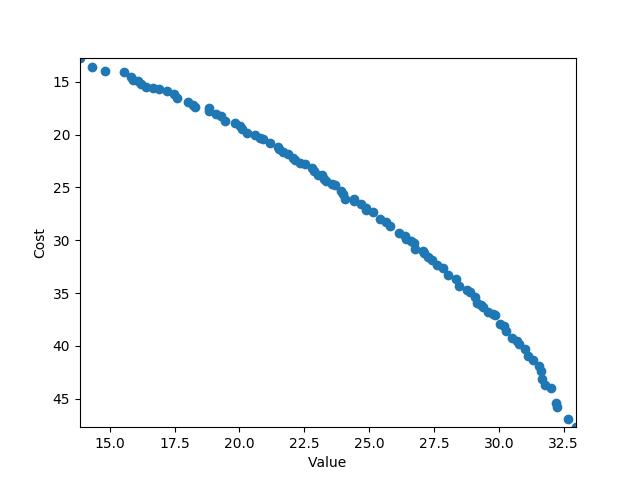
\includegraphics[width=\linewidth]{res/multi_obj.png}

\subsubsection{Single Objective Genetic Algorithm}
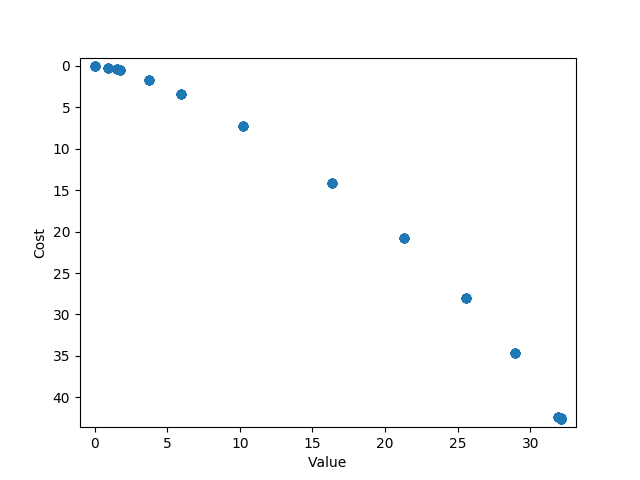
\includegraphics[width=\linewidth]{res/single_obj.png}

\subsubsection{Random Search}
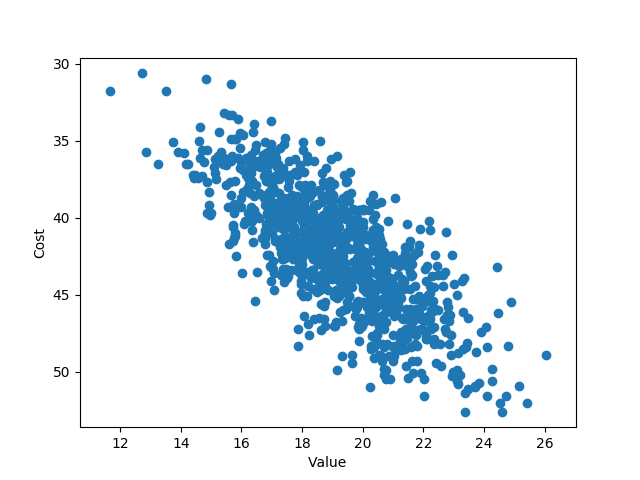
\includegraphics[width=\linewidth]{res/random.png}

\subsection{Realistic NRP Dataset}
\subsubsection{NSGA-II}
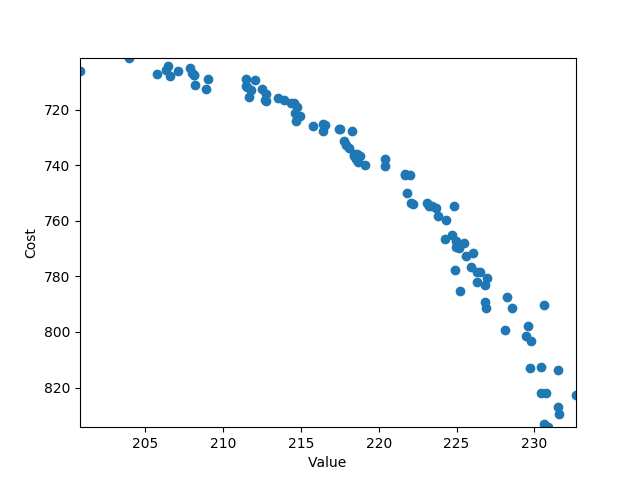
\includegraphics[width=\linewidth]{res/multi_obj_real.png}

\subsubsection{Single Objective Genetic Algorithm}
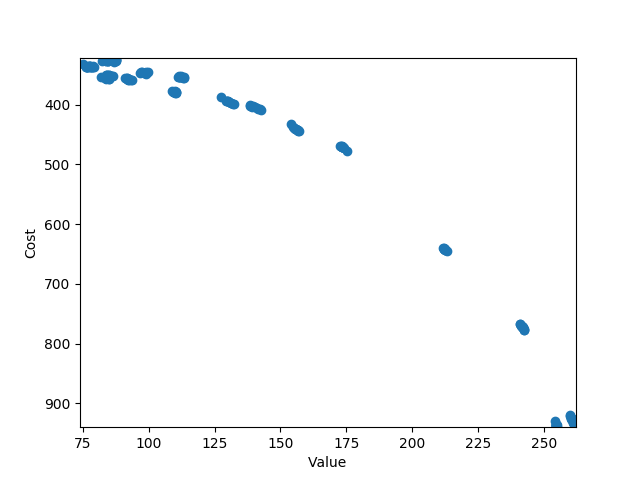
\includegraphics[width=\linewidth]{res/single_obj_real.png}

\subsubsection{Random Search}
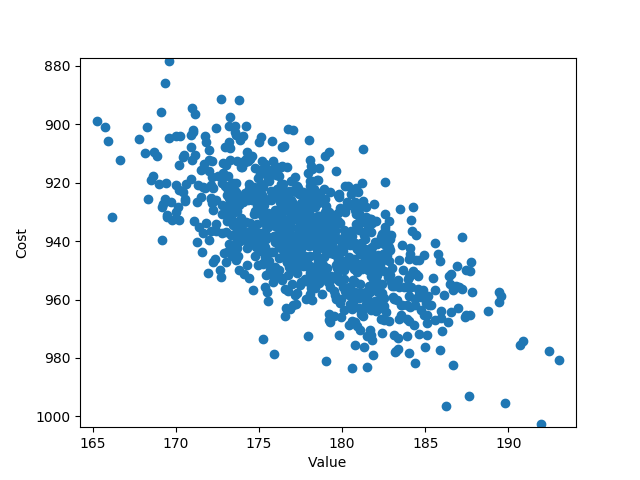
\includegraphics[width=\linewidth]{res/random_real.png}


\section{Analysis}
\subsection{Classic NRP Dataset}
\subsubsection{NSGA-II}
As expected, the NSGA-II provided an evenly-distributed pareto front of solutions that show the tradeoff between the value and cost of each set of requirements.

\subsubsection{Single Objective Genetic Algorithm}
The single objective genetic algorithm produced a similar graph to the NSGA-II algorithm, however the solutions are clustered much closed together. This is likely due the the fact that some viable optimal solutions are not scored as highly in the single-objective evaluation function. The single objective GA is clearly inferior for this problem domain, as many of the solutions it misses are viable and could be more optimal on a case-by-case bases than the ones it finds.

\subsubsection{Random Search}
The random search performed poorly on this problem, as expected. In includes solutions which are dominated, and fails to find results at either extreme.

\subsection{Realistic NRP Dataset}
\subsubsection{NSGA-II}
In comparison to the classic dataset, the realistic dataset produced a much more noisy pareto front. This is presumably due to certain values of cost and value not being reachable, as well as having much more data to work on. I theorise it could be improved by increasing the number of iterations, but the current results are most likely "good enough".

\subsubsection{Single Objective Genetic Algorithm}
In comparison to the classic dataset, the single objective genetic algorithm produced much worse results when ran on the realistic dataset. There was a slightly wider spread of results which is to be expected when using more data, however the results than were generated were far inferior to those generated by the NSGA-II algorithm. Also of note is the time taken to run the single objective genetic algorithm - it took over 3 hours to produce a dataset, which is still far longer for an individual run than the NSGA-II algorithm took.

\subsubsection{Random Search}
As expected, the random search performed dismally on this dataset as well - dominated solutions are included, and the best solutions have far higher costs for their value when compared to either of the other algorithms.

\end{document}